\section{Background}\label{sec:background} 
\begin{figure}[t]
  \centering
  \vspace{2mm}
  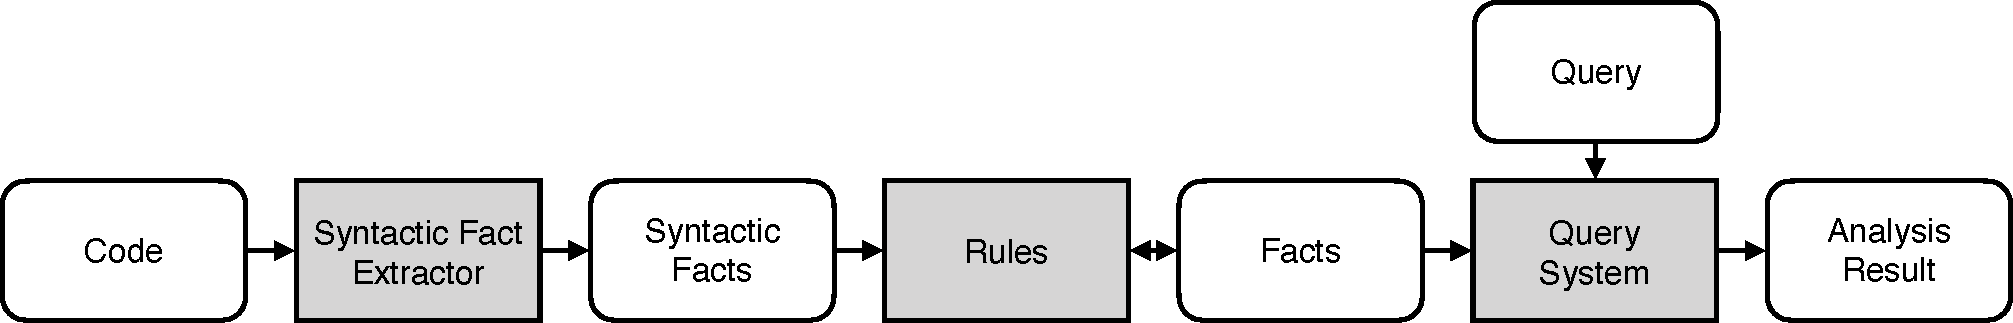
\includegraphics[width=0.94\textwidth]{img/ov1.pdf}
%  \vspace*{-1.5em}
  \caption{Overview of a declarative static analysis}
  \label{fig:ov1}
%\vspace*{-.5em}
\end{figure}

Figure~\ref{fig:ov1} presents the overview of how a declarative static
analysis works.  The analysis consists of three steps.  First, a given program
gets converted into syntactic facts. \inred{ Second, new facts are generated by iteratively applying
rules to the set of known facts, until no new facts are derived.}  Finally,
the query system takes a query and evaluates the rules with the
given facts, producing an analysis result for the query. \inred{The following paragraphs
explain each steps in detail, using examples with datalog-like syntax.}

%Figure~\ref{fig:ov1} presents the overview of how a declarative style analysis
%works. The analysis consists of three steps.  First, a given program gets
%converted into database of syntactic facts.  Second, the rules that generate
%new facts are defined, and a declarative language engine evaluates the rules
%with the given facts, producing new facts.  Finally, the query is executed to
%extract all the facts that meet certain conditions, which correspond to the
%analysis result.

\textbf{Step 1: Extracting syntactic facts.}
The first step is to extract syntactic facts from a given program source.
Syntactic facts include facts about certain AST nodes and
parent-child relationships between nodes. For example, consider
the following code:

\begin{lstlisting}[style=mcpp]
int f() {
  return 42;
}

int val = f();
\end{lstlisting}
\inred{The extractor can extract the syntactic facts} of the form \inred{\rcode{ FunctionAt(lineNum, name)}}, where
\inred{\rcode{ lineNum}} denotes the line number and \rcode{ name} denotes the name of the function
defined at line \inred{\rcode{ lineNum}}.  Therefore, we can extract the fact \rcode{
FunctionAt(1, "f")}.  Another example syntactic fact is \inred{\rcode{ EnclosingStmt(lineNum1,
lineNum2, i)}}, which denotes that the function at line \inred{\rcode{ lineNum1}} has the statement
at line \inred{\rcode{ lineNum2}} as the \rcode{ i}-th statement in the function body.  For
example, we can extract the following syntactic fact: \rcode{ EnclosingStmt(1, 2,
0)}.

These syntactic facts serve as building blocks for the
common Intermediate Representation (IR) of multiple languages.
Compared to other IRs, this declarative-style IR has a few advantages.
First, extracting information from source code in this format does not
require any understanding of the language semantics, which imposes
almost no performance overhead beyond parsing the source code.
Second, the syntactic facts can be utilized easily in other kinds of
analysis, since they are simple information that can be freely
manipulated when defining new rules. Therefore, even when we use a different
client analysis, we can reuse the extracted syntactic facts
without re-extracting them from the source code.

\smallskip
\textbf{Step 2: \inred{Deriving new facts using rules.}}
\inred{
The next step is to derive new facts out of known facts, using rules.
One rule indicates that if a certain facts are known, then a new rule can be
generated and added to the set of known facts. This process of generating
new facts is repeated, until no more new facts are found.
}

For example, \inred{ consider the dataflow
analysis fact \rcode{ Flow(x, z)},  which denotes that there is a dataflow from a node \rcode{ x}
to a node \rcode{ z}. Here, nodes} represent program entities that can hold
run-time values, such as variables, literals, and function parameters.  We
can \inred{consider} a rule for generating this fact as the transitive closure of the fact named
\rcode{ Step}:

\begin{lstlisting}[style=mrule]
Flow(x, z) :- Step(x, z)
Flow(x, z) :- Step(x, y), Flow(y, z)
\end{lstlisting}

\noindent
where \rcode{ Step(x, z)} denotes a single direct dataflow from \rcode{ x} to \rcode{ z}. \inred {This
rule indicates that a new fact \rcode{ Flow(x, z)} can be derived, if there is a fact \rcode{ Step(x, z)} or
there two facts \rcode{ Step(x, y)} and \rcode{ Flow(y, z)} in the set of known facts. A new fact
generated in this way will be added to the set of known facts, and can be utilized to derive yet another fact. }
\inred{ \sout {
The rules are usually
evaluated in a bottom-up and modular manner, that is, each rule is evaluated
one by one, after every rule it depends on is evaluated.
}}

%The next step is to define rules to generate new facts out of known facts.
%%This step corresponds to actually implementing the algorithm of a
%%static analysis in a declarative style.
%For example, recall that we can define a call graph
%\rcode{ CallEdge(l1, l2)} using the facts
%named \rcode{ FunctionAt} and \rcode{ CallAt}.
%The defined rules are evaluated with declarative engines to finding all possible
%facts that can be derived. The rules are usually evaluated in a bottom-up
%and modular manner. Each rule is evaluated one-by-one, after every
%rule it depends on is evaluated. 

\smallskip
\textbf{Step 3: Performing queries.}
The final step is to perform the query via the query system.  A query \inred{is}
a set of facts containing variables, and the query system finds every variable
assignment that makes all of \inred{substituted facts in the query to be included in the
derived set of known facts.}
This step corresponds to actually obtaining the
final result of a static analysis in a declarative style.
For example, one can make a specific query:

\begin{lstlisting}[style=mrule]
?- Flow(42, X)
\end{lstlisting}

\noindent
that queries all nodes into which the integer literal {\tt 42} flows.
When accepting the query as an input, the query system finds 
\inred{
every value \rcode{ v} such that \rcode{ Flow(42, v)} is included in
the set of know facts, generated in the previous step. In this example, the query would give the query result
\rcode{ X = 42}, \rcode{ X = f()} and \rcode{ X = val}.}

%The final step is to perform queries via query system.
%The result of the query corresponds to actual result of client analysis.
%A query consists of set of facts, where some of the facts would have
%varaibles as arguments. Given a query, the query sytem will find all possible
%assignment on variables, that will make every facts would hold under
%the assignment.
%\newpage
